%%%%%%%%%%%%%%%%%%%%%%%%%%%%%%%%%%%%%%%%%
% Beamer Presentation
% LaTeX Template
% Version 1.0 (10/11/12)
%
% This template has been downloaded from:
% http://www.LaTeXTemplates.com
%
% License:
% CC BY-NC-SA 3.0 (http://creativecommons.org/licenses/by-nc-sa/3.0/)
%
%%%%%%%%%%%%%%%%%%%%%%%%%%%%%%%%%%%%%%%%%

%----------------------------------------------------------------------------------------
%	PACKAGES AND THEMES
%----------------------------------------------------------------------------------------

\documentclass{beamer}

\mode<presentation> {

% The Beamer class comes with a number of default slide themes
% which change the colors and layouts of slides. Below this is a list
% of all the themes, uncomment each in turn to see what they look like.


%\usetheme{Luebeck}
\usetheme{Madrid}
%\usetheme{Malmoe}
%\usetheme{Marburg}
}

% As well as themes, the Beamer class has a number of color themes
% for any slide theme. Uncomment each of these in turn to see how it
% changes the colors of your current slide theme.

%

%\setbeamertemplate{footline} % To remove the footer line in all slides uncomment this line
%\setbeamertemplate{footline}[page number] % To replace the footer line in all slides with a simple slide count uncomment this line

%\setbeamertemplate{navigation symbols}{} % To remove the navigation symbols from the bottom of all slides uncomment this line
\usepackage{xspace}
\usepackage{amsmath,mathrsfs,amscd}
\usepackage{subfig}
\usepackage{slashed}
\usepackage{graphicx} % Allows including images
\usepackage{booktabs} % Allows the use of \toprule, \midrule and \bottomrule in tables
\usepackage[compat=1.1.0]{tikz-feynman}
\newcommand\Tstrut{\rule{0pt}{3.0ex}}         % = `top' strut
\newcommand\Bstrut{\rule[-1.5ex]{0pt}{0pt}}   % = `bottom' strut
\newcommand{\ftapprox}{FT$_{\mathrm{approx}}$\xspace}
\newcommand{\nnloBP}{NNLO$_{\mathrm{B-proj}}$\xspace}
\newcommand{\nnloNI}{NNLO$_{\mathrm{NLO-i}}$\xspace}
\newcommand{\nnloFT}{NNLO$_{\mathrm{FTapprox}}$\xspace}
\newcommand{\nloFT}{NLO$_{\mathrm{FTapprox}}$\xspace}
\newcommand{\sqrtS}{\ensuremath{\sqrt{s}}}
\def\E#1{\times 10^{#1}}

%----------------------------------------------------------------------------------------
%	TITLE PAGE
%----------------------------------------------------------------------------------------

\title[tth]{Measure Higgs CP via tth Channel} % The short title appears at the bottom of every slide, the full title is only on the title page

\author{Ren-Qi Pan} % Your name
\institute[ZJU] % Your institution as it will appear on the bottom of every slide, may be shorthand to save space
{
Zhejiang Institute of Modern Physics\\ % Your institution for the title page
\medskip
\textit{renqipan@zju.edu.cn} % Your email address
}
%\date{\today} % Date, can be changed to a custom date
\pagenumbering{arabic}

\begin{document}

\begin{frame}
\titlepage % Print the title page as the first slide
\end{frame}

\begin{frame}
\frametitle{Overview} % Table of contents slide, comment this block out to remove it
\tableofcontents % Throughout your presentation, if you choose to use \section{} and \subsection{} commands, these will automatically be printed on this slide as an overview of your presentation
\end{frame}

%----------------------------------------------------------------------------------------
%	PRESENTATION SLIDES
%----------------------------------------------------------------------------------------

%------------------------------------------------
\section{Towards Machine Learning}
\begin{frame}
\frametitle{Machine Learning}

\begin{figure}
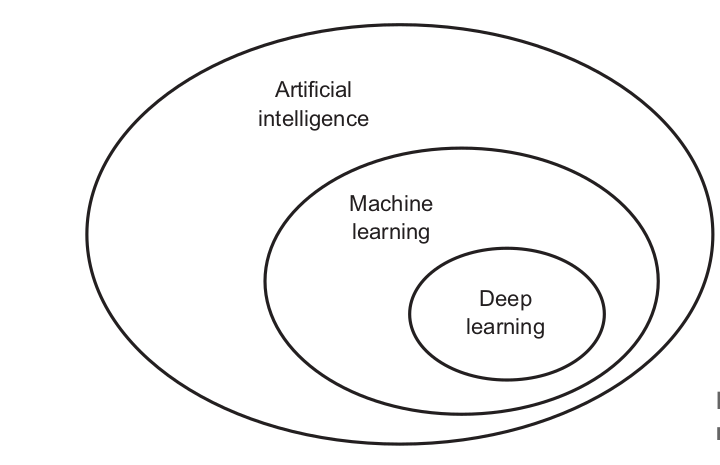
\includegraphics[scale=0.15]{./figures/Al}
\caption{Artificial intelligence}
\end{figure}

\begin{figure}
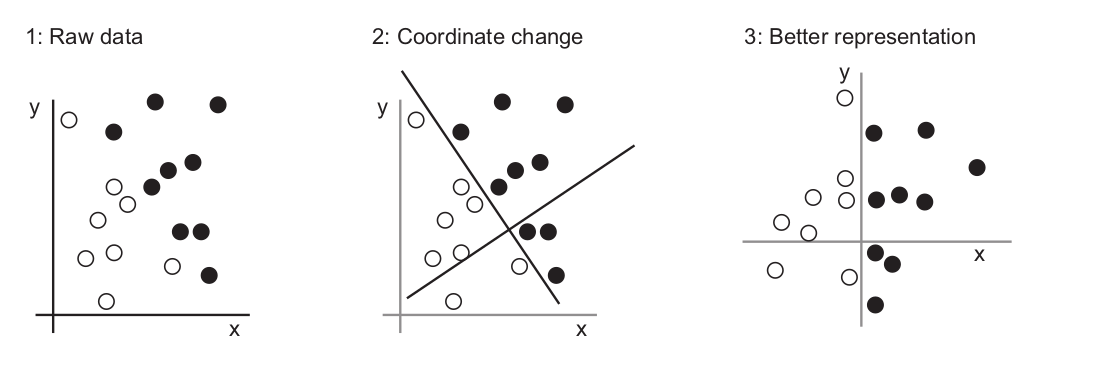
\includegraphics[scale=0.20]{./figures/rep}
\caption{Coordinate change. Learning, in the context of machine learning, \ describes an automatic search
process for better representations.}
\end{figure}
\end{frame}

\begin{frame}
\frametitle{Common Models of Machine Learning}
\begin{itemize}
\item Support vector machines
\item Bayesian networks
\item Boosting decision trees: AdaBoost, Gradient Boosting, XGBoost
\item Artificial neural network
\end{itemize}
\end{frame}
\subsection{Decision tree}
\begin{frame}
\frametitle{Decision tree}
\begin{figure}[right]
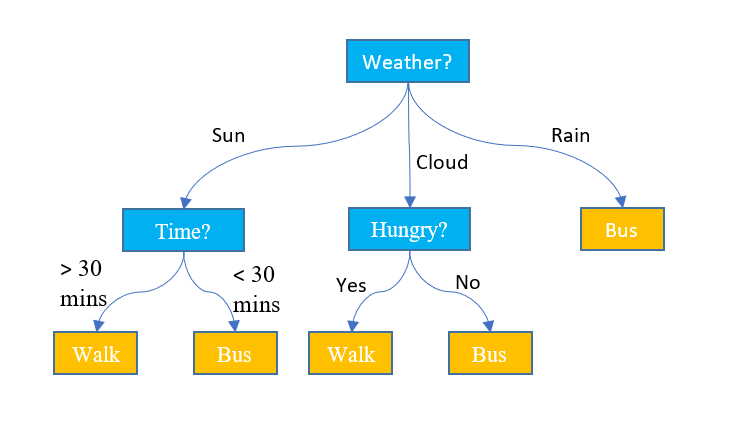
\includegraphics[scale=0.23]{./figures/decision.png}
\caption{A decision tree}
\end{figure}
A decision tree takes a set of input features and splits input data
recursively based on those features.
\begin{itemize}
\item Nodes
\begin{itemize}
\item The data is split based on a value of one of features at each node.
\item Sometime called “interior nodes”
\end{itemize}
\item Leaves
\begin{itemize}
\item Terminal nodes
\item Represent a class label or probability
\item If the outcome is a continuous variable it’s considered a “regression tree”
\end{itemize}
\end{itemize}
\end{frame}

\begin{frame}
\frametitle{Decision tree}
Learning:
\begin{itemize}
\item Each split at a node is chosen to maximize information gain(rate)
\item The splits are created recursively
\end{itemize}
Note:
\begin{itemize}
\item Information gain is the difference in entropy before and after the potential split
\item The process is repeated until some stop condition is met.
Ex: depth of tree, no more information gain, etc...
\end{itemize}
\end{frame}

\begin{frame}
\frametitle{Information Gain}
 category information entropy: 
\begin{equation*}
Info(D)=-\sum_{i}^{m} p_i log_2(p_i)
\end{equation*}
feature information entropy:
\begin{equation*}
Info_{A}(D)=\sum_{j=1}^{v}\frac{\vert D_j \vert}{\vert D\vert}*Info(D_j)
\end{equation*}
information gain: $Gain(A)=Info(D)-Info_{A}(D)$
\end{frame}


\begin{frame}
\frametitle{Information Gain Rate}
 feature splitting information entropy: 
\begin{equation*}
SplitInfo_{A}(D)=-\sum_{j=1}^{v}\frac{\vert D_j \vert}{\vert D\vert} log_{2}\frac{\vert D_j \vert}{\vert D\vert}
\end{equation*}
information gain rate:
\begin{equation*}
GainRate(A)=\frac{Gain(A)}{SplitInfo_{A}(D)}
\end{equation*}
\end{frame}
\subsection{Boosting decision tree}
\begin{frame}
\frametitle{Boostin decision tree}
Usually, a single tree is not strong enough to be used in practice. What is actually used is the ensemble model, which sums the prediction of multiple trees together.
\begin{figure}
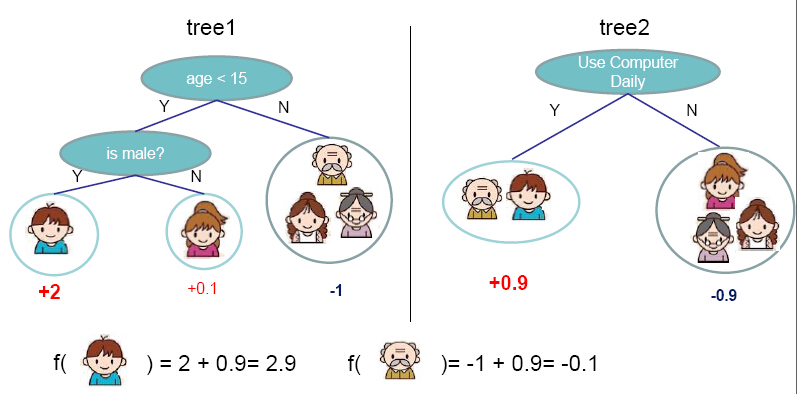
\includegraphics[scale=0.40]{./figures/boosting}
\caption{Here is an example of a tree ensemble of two trees. The prediction scores of each individual tree are summed up to get the final score}
\end{figure}
\end{frame}
\begin{frame}
\frametitle{Tree boosting}
Boosting is a method of combining many weak learners (trees) into a strong classifier.
\begin{itemize}
\item Each tree is created iteratively
\item The tree’s output (h(x)) is given a weight (w) relative to its accuracy
\item Use residual to create a new tree
\item The ensemble output is the weighted sum:  $\hat{y}=\sum_{t}w_{t} h_{t}(x)$
\item After each iteration each data sample is given a weight based on its misclassification\\
Note: The more often a data sample is misclassified, the more important it becomes 
\item The goal is to minimize an objective function
\end{itemize}
\end{frame}

\begin{frame}
\frametitle{Types of boosting}
There are many different ways of iteratively adding learners to minimize a loss function.
Some of the most common:\\
\begin{itemize}
\item AdaBoost
\begin{itemize}
\item “Adaptive Boosting”
\item One of the originals
\item residual=prediction- real value 
\end{itemize}

\item Gradient Boosting
\begin{itemize}
\item Uses gradient descent to create new learners
\item The loss function is differentiable 
\item residual: minus gradient of loss function
\end{itemize}

\item XGBoost
\begin{itemize}
\item “eXtreme Gradient Boosting”
\item Type of gradient boosting
\item Objective Function: Training Loss + Regularization
\item Taylor expansion of the loss function up to the second order
\item Shrinkage and Column Subsampling
\end{itemize}
\end{itemize}
\end{frame}

\subsection{Keras-DNN}
\begin{frame}
\frametitle{Keras and TensorFlow}
Keras:
\begin{itemize}
\item model-level library(released in 27 March 2015)
\item an open-source neural-network library written in Python
\item providing high-level building blocks for developing deep-learning models
\end{itemize}
TensorFlow:
\begin{itemize}
\item TensorFlow is developed by Google(released in  November 9, 2015)
\item serving as the backend engine of Keras
\item handle low-level operations such as tensor manipulation and differentiation
\end{itemize}
\end{frame}

\begin{frame}
\frametitle{Mechanism of DNN}
\begin{figure}[H]
\centering
\subfloat[mechanism of artificial neural network] {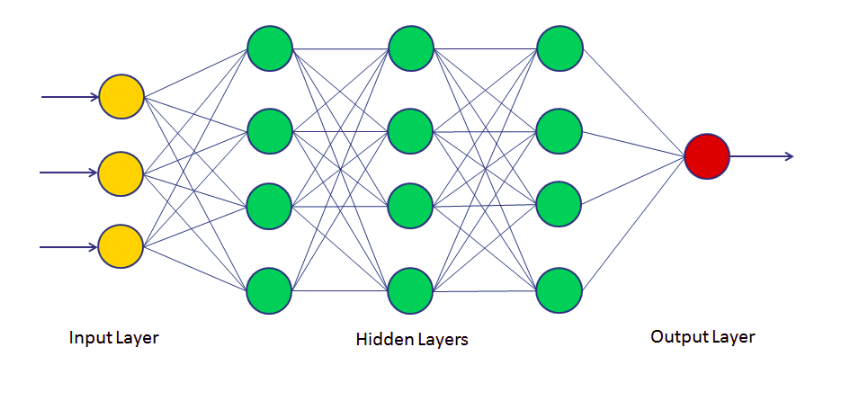
\includegraphics[width=0.5\textwidth]{./figures/neural.png}} 
\subfloat[Here’s a diagram of what one node might look like.]{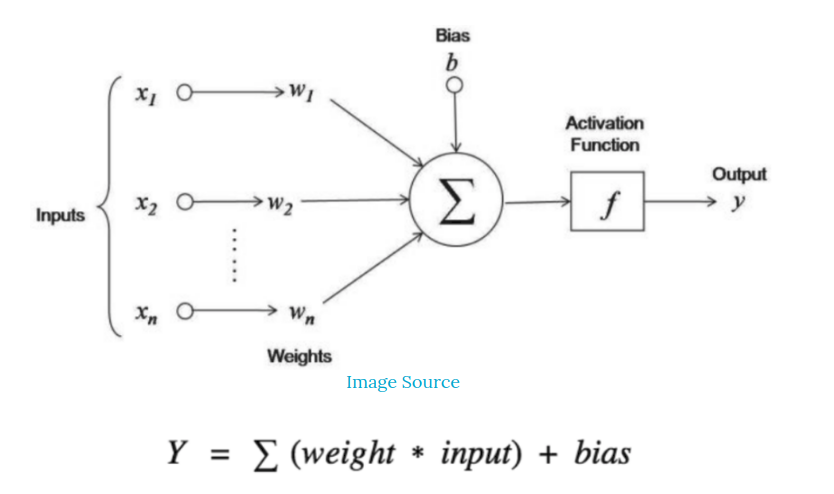
\includegraphics[width=0.5\textwidth]{./figures/layer.png}}
\end{figure}
\end{frame}


\begin{frame}
\frametitle{Activation function}
\begin{figure}
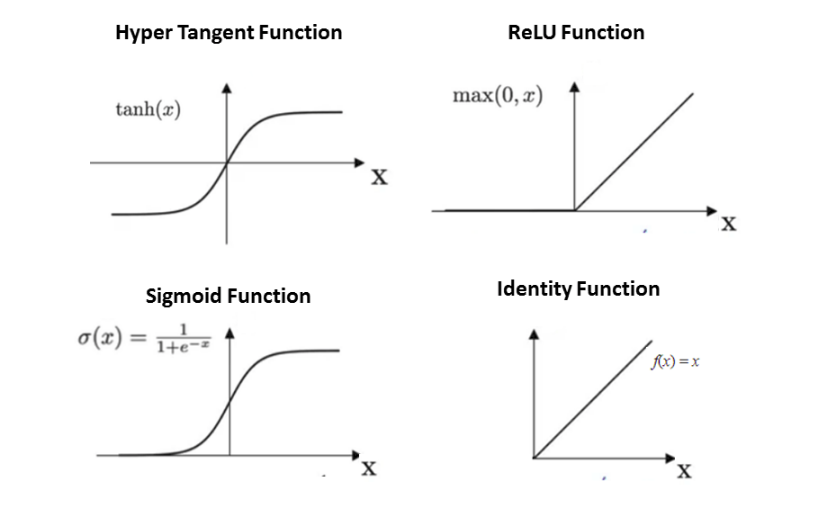
\includegraphics[scale=0.35]{./figures/activation.png}
\caption{common activation function used in artificial neural network.}
\end{figure}
\end{frame}

\begin{frame}
\frametitle{Components of neural network}
Training a neural network revolves around the following objects:
\begin{itemize}
\item \textbf{Layers}, which are combined into a network (or model)
\item The \textbf{input data} and corresponding \textbf{targets}
\item The \textbf{loss function}, which defines the feedback signal used for learning
\item The \textbf{optimizer}, which determines how to update weights
\end{itemize}
\end{frame}

\begin{frame}
\frametitle{How neural network work?}
\begin{figure}
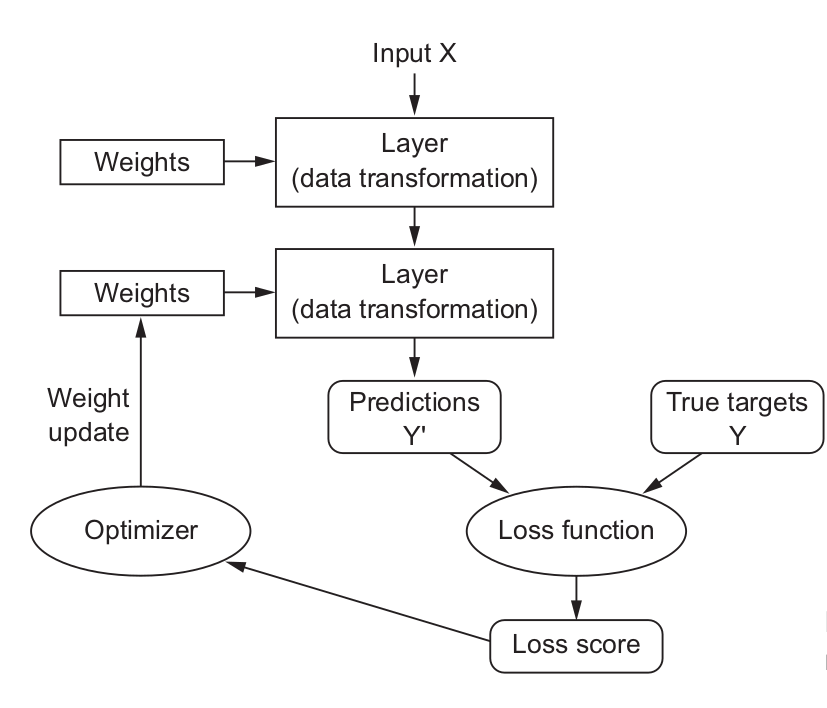
\includegraphics[scale=0.25]{./figures/interaction.png}
\caption{Relationship between the network, layers, loss function, and optimizer}
\end{figure}
\end{frame}

\begin{frame}
\frametitle{An neural network model}
\begin{figure}
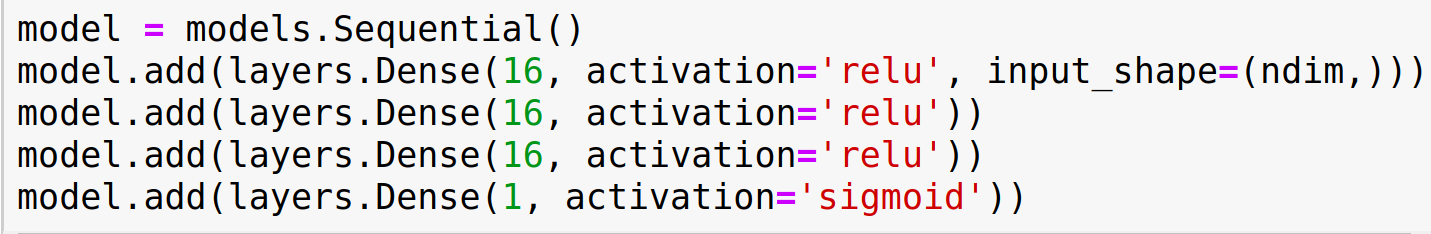
\includegraphics[scale=0.25]{./figures/model.png}
\caption{An example of artificail neural network model with 4 layers.}
\end{figure}
\end{frame}


\section{Apply Machine Learning to Measure Higgs CP via tth}

\subsection{Determine input variables}
\begin{frame}
%\frametitle{Higgs boson decay}
\begin{figure}[H]
\centering
\subfloat[compare the ROC curve between with and without btag]{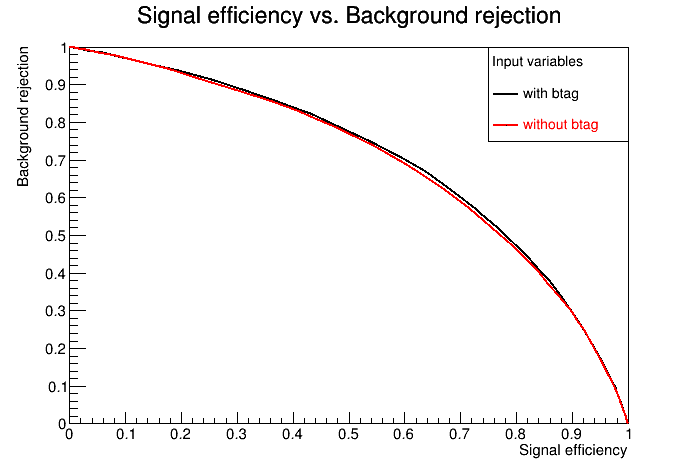
\includegraphics[width=0.5\textwidth]{./figures/ROC_Curve_btag.png}} 
\subfloat[ compare the ROC curve between 6 jets and 10 jets]{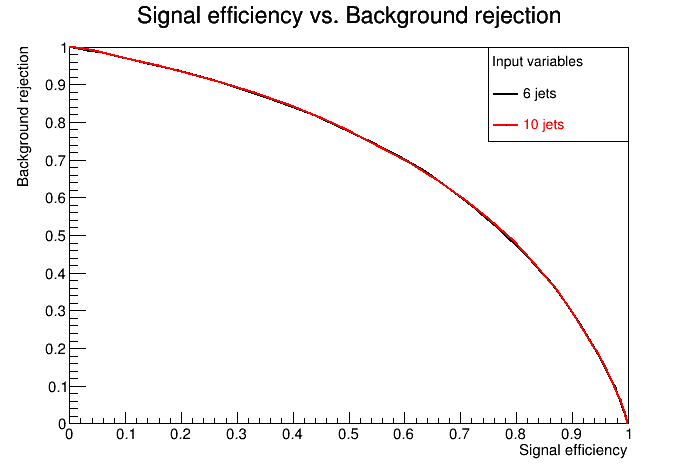
\includegraphics[width=0.5\textwidth]{./figures/ROC_Curve_jets.png}}
\end{figure}
\end{frame}

\begin{frame}
%\frametitle{Higgs boson decay}
\begin{figure}[H]
\centering
\subfloat[diphoton information vs. 2 photons information]{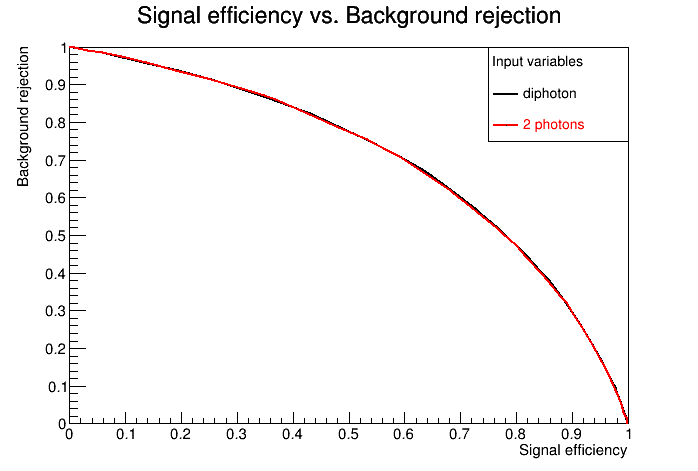
\includegraphics[width=0.5\textwidth]{./figures/ROC_Curve_photon.png}} 
\subfloat[ with or without diPhoMass]{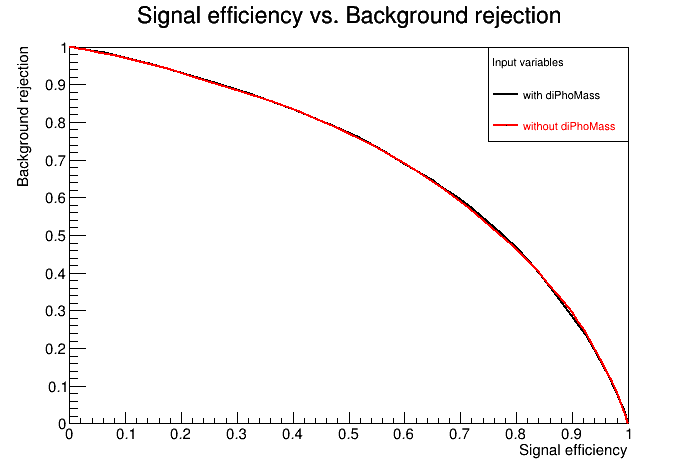
\includegraphics[width=0.5\textwidth]{./figures/ROC_Curve_diphomass.png}}
\end{figure}
\end{frame}


\begin{frame}
\frametitle{Different input variables}
\begin{figure}
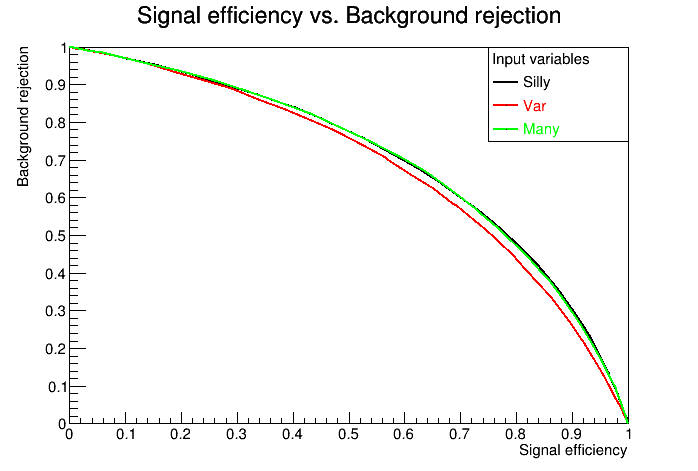
\includegraphics[scale=0.25]{./figures/ROC_Curve3.png}
\caption{compare the ROC curve between three different types of input variables.}
\end{figure}
\end{frame}

\begin{frame}
\frametitle{Input variables}
From here on the input variables are :
\begin{itemize}
\item 6 jets: Pt,  E,  Eta, Phi, btag
\item diPhoPhi, diPhoEta, diPhoPtoM
\item in total 33 variables
\end{itemize}
\begin{figure}
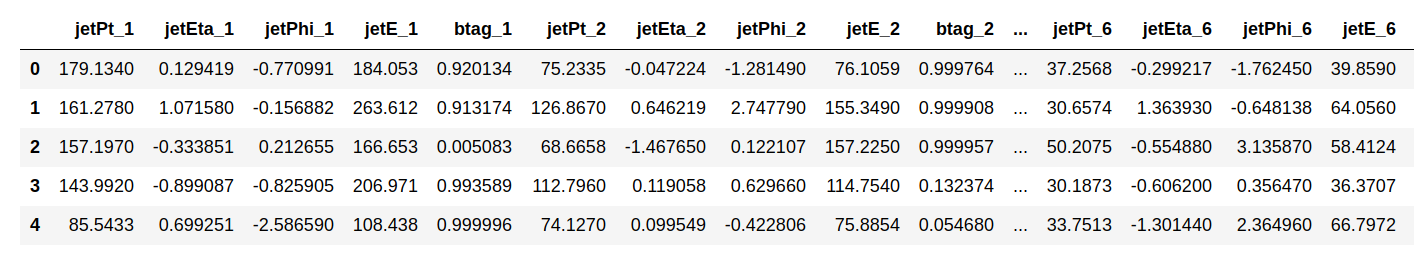
\includegraphics[scale=0.25]{./figures/input.png}
\caption{partial input data}
\end{figure}
\end{frame}
\subsection{Response value and ROC curve}
\begin{frame}
\frametitle{TMVA response for classifier: AdaBoost}
\begin{figure}
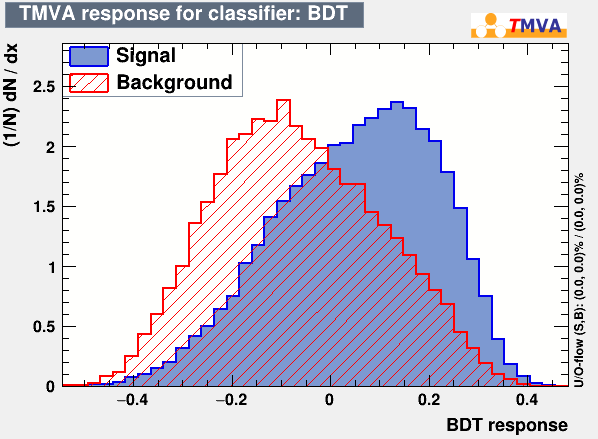
\includegraphics[scale=0.25]{./figures/mva_BDT.png}
\caption{TMVA-AdaBoost response under Higgs CP even and odd.}
\end{figure}
\end{frame}

\begin{frame}
\frametitle{xgboost and DNN}
\begin{figure}[H]
\centering
\subfloat[xgboost response]{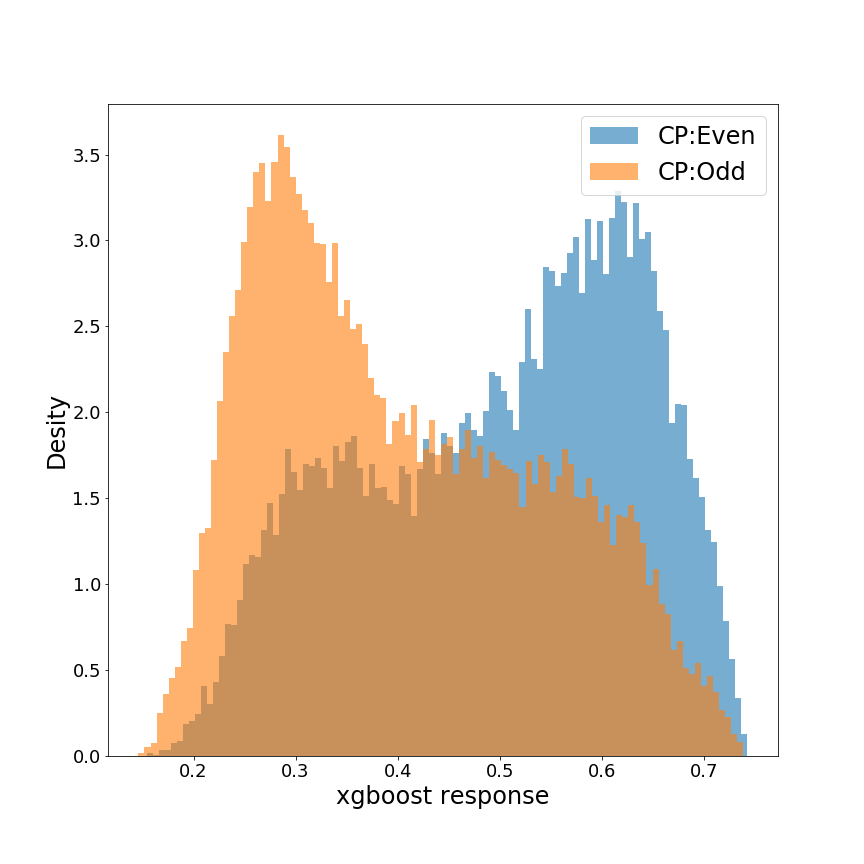
\includegraphics[width=0.5\textwidth]{./figures/tth_xgboost_output.png}} 
\subfloat[keras-DNN response]{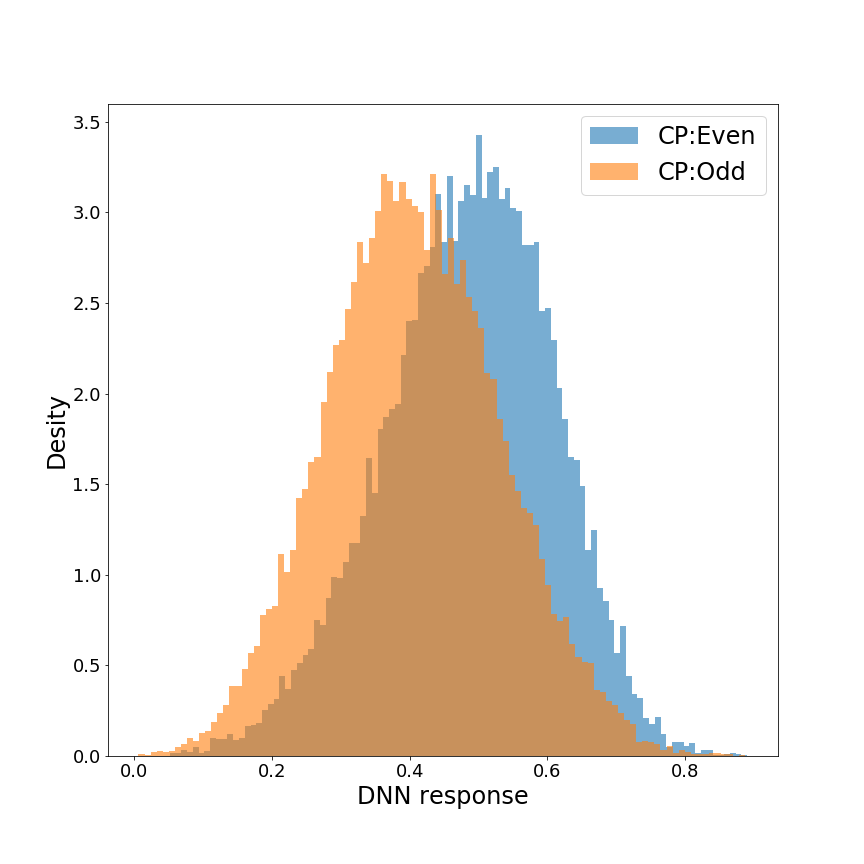
\includegraphics[width=0.5\textwidth]{./figures/tth_keras_output.png}}
\end{figure}
\end{frame}

\begin{frame}
\frametitle{Different models}
\begin{figure}
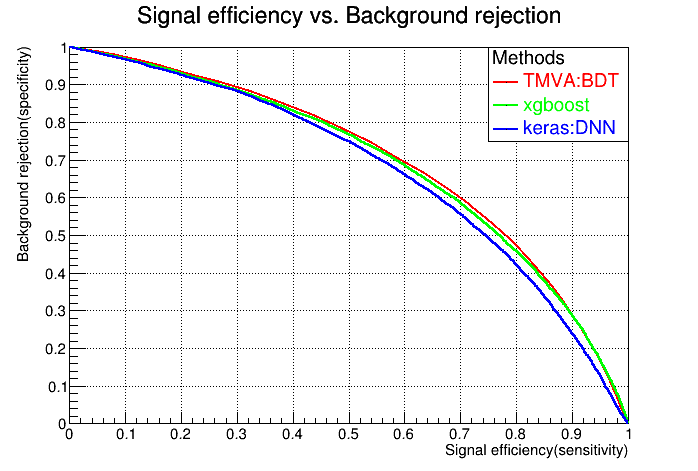
\includegraphics[scale=0.25]{./figures/tmva_xgboost.png}
\caption{compare the ROC curves of three different models.}
\end{figure}
\end{frame}






%------------------------------------------------

\begin{frame}
\Huge{\centerline{The End}}
\end{frame}

%----------------------------------------------------------------------------------------

\end{document} 